\section{Implementation Details}
\subsection{Object Proposals}
We use MCG object proposals in~\cite{arbelaez2014multiscale} as object candidates. Since the object proposals mainly covers the objects,  we also generate a small number (20$\sim$30 per image) of segments using the stable segmentation algorithm from~\cite{chen2011piecing} to cover the whole scene including contextual classes. To reduce the computational overhead, our context voting step uses only the stable segments. The stable segmentation gives a coarse level of object/context division and reduces the computational complexity of context voting compared to the large number of finer object proposals, while still maintaining a semantically informative contextual inference. 

\subsection{Datasets}
We conduct our training and experiments on the Pascal VOC dataset.~\cite{Everingham10} which is a \textit{de facto} benchmark for object detection. Since the original dataset does not provide annotation of segmentation and contextual classes, we train our policy using the Pascal Context dataset~\cite{mottaghi2014role} which fully annotates every pixel of the Pascal VOC 2010 train and validation sets, with additional contextual classes such as sky, grass, ground, building etc., which is adequate for our purposes. We use the 33 context classes from~\cite{mottaghi2014role} and train our policy on the Pascal Context training set, and test our algorithm and baselines on the validation set. We also test our policy on the MSRC dataset~\cite{shotton2006textonboost} to show our algorithm can generalize to different data. 

\subsection{Feature Representation}
To classify object proposals, we extract region features and classify them using the deep neural network model in~\cite{BharathECCV2014} fine-tuned on Pascal VOC 2012. For the policy action classifiers, we also use the same model to extract features for states represented by the masks of search area $X^t$ and observed area $O^t$ in state $s_t$, then concatenate the features as inputs to the policy. For context classifiers we use a subset of the appearance features for superpixels from~\cite{tighe2010superparsing} and learn one-vs-all SVM models for classification.

\section{Experiments}

We conduct our experiments on the Pascal VOC 2010 dataset, in consistence with the data to train our context model. We evaluate the object detection performance by mean average precision (mAP). Since we also evaluate the performance of simultaneous detection and segmentation, we use the validation set as our test set which provides object segmentation annotations. 

%\subsection{Reduction of Number of Object Proposals}

\begin{figure}[htb!]
\begin{center}
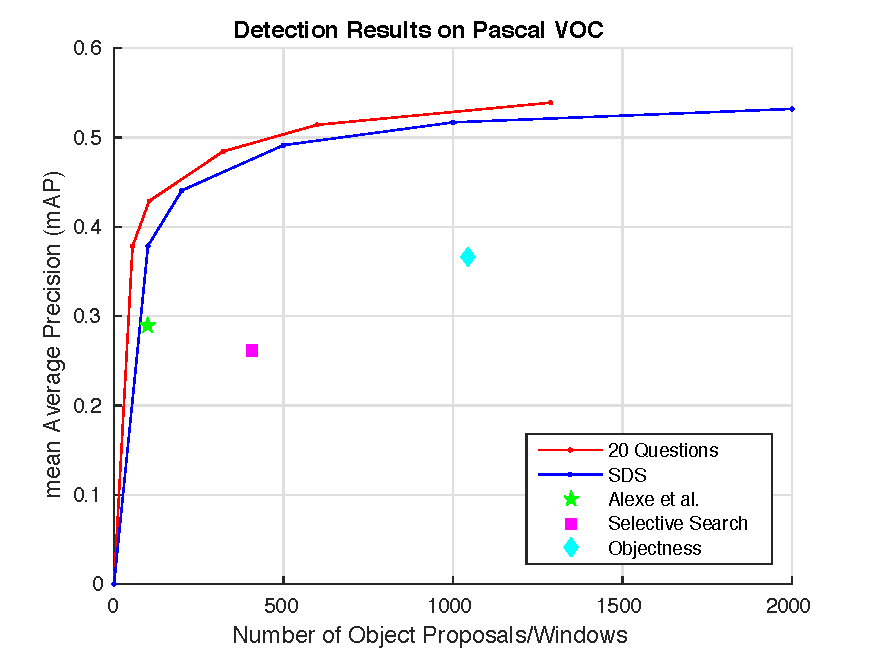
\includegraphics[width=0.6\linewidth]{figures/numprop.pdf}
\end{center}
\caption{Performance on Pascal VOC dataset. Best viewed in color. }
\label{fig:mapVSnumprop}
\end{figure}

%%%%%%%%%%%%%%%%%%%%%%%%%%%%%%%%%%%
{\bf Reduction of Number of Object Proposals} 
Figure~\ref{fig:mapVSnumprop} shows the average precision performance on the Pascal VOC 2010 dataset with respect to the number of object proposals/windows used. We compared our 20 question approach to the baseline of running detectors in~\cite{BharathECCV2014} exhaustively over all object proposals,  window selection driven by context in~\cite{bogdan2012context}, detection using object proposals in selective search~\cite{van2011segmentation} and objectness~\cite{alexe2010object}. We can see that that our 20 questions detection algorithm can effectively reduce a large amount of object proposals ($30\% \sim 40\%$) with little loss compared to exhaustive detection on all object proposals.  Thus our approach can achieve comparable results with much less object proposals and corresponding detector evaluation. Our approach has also outperformed random search approach which randomly samples the same number of object proposals for detection. With the increase of the number of object proposals, our algorithm can even gain improvement due to the reduction of false positives. 

%%%%%%%%%%%%%%%%%%%%%%%%%%%%%%%%%%%%%

{\bf Comparison with context based methods} We compare our model with the SDS exhaustive search baseline and a recent proposed contextual model in~\cite{mottaghi2014role}, which considers global and local context in a Markov Random Field framework based on deformable part-based model. This model has high computational cost since it needs to evaluate hundreds of thousands of windows as well as the context deformation term between all context boxes in the graph. Table~\ref{Tablepascal} shows the classwise mAP of our 20 questions-based object detection with other context based methods and their corresponding baselines.  Our 20 question detection approach has outperformed the SDS exhaustive search baseline as well as DPM based context approaches. The initial object proposal number is 2000 for both the SDS and the 20 question method; after the 20 questions refinement of the search space the average number of detector evaluations (including the overhead of context classifiers evaluated) has decreased 36\%. We can see that although there are performance drops in some classes due to possible rejection of true object candidates, for some classes that are closely related in some types of scenes such as car, boat, 


\begin{table*}\tiny
\caption{Avg. Precision for detection of our algorithm against previous contextual approaches on PASCAL VOC10 dataset.}
\begin{tabular}{p{1.60cm}|p{0.144cm}p{0.144cm}p{0.144cm}p{0.144cm}p{0.144cm}p{0.144cm}p{0.144cm}p{0.144cm}p{0.144cm}p{0.144cm}p{0.144cm}p{0.144cm}p{0.144cm}p{0.144cm}p{0.144cm}p{0.144cm}p{0.144cm}p{0.144cm}p{0.144cm}p{0.144cm}p{0.144cm}c}
&{\begin{sideways}Aeroplane\end{sideways}}&{\begin{sideways}Bicycle\end{sideways}}&
{\begin{sideways}Bird\end{sideways}}&{\begin{sideways}Boat\end{sideways}}&{\begin{sideways}Bottle\end{sideways}}&{\begin{sideways}Bus\end{sideways}}
&{\begin{sideways}Car\end{sideways}}&{\begin{sideways}Cat\end{sideways}}&{\begin{sideways}Chair\end{sideways}}&{\begin{sideways}Cow\end{sideways}}
&{\begin{sideways}Dining Table\end{sideways}}&{\begin{sideways}Dog\end{sideways}}&{\begin{sideways}Horse\end{sideways}}&{\begin{sideways}Motor Bike\end{sideways}}&{\begin{sideways}Person\end{sideways}}
&{\begin{sideways}Potted Plant\end{sideways}}&{\begin{sideways}Sheep\end{sideways}}&{\begin{sideways}Sofa\end{sideways}}&{\begin{sideways}Train\end{sideways}}&{\begin{sideways}TV/Monitor\end{sideways}}
&{\begin{sideways}Average\end{sideways}}\\
DPM & 44.3 & 51.3 & 7.1 & 8.0 & 21.8 & 56.0 & 41.2 & 18.4 & 13.8 & 11.7 & 10.4 & 13.5 & 38.3 & 42.7 & 44.6 & 3.7 & 27.0 & 24.3 & 38.0 & 32.2 & 27.4 \\                                  
\hline                                                                                                                                                                                  
DPM + 33 Context & 46.4 & 50.8 & 7.5 & 8.2 & 21.2 & 55.3 & 41.6 & 20.0 & 14.7 & 11.8 & 11.6 & 13.9 & 37.9 & 40.2 & 45.1 & 4.2 & 24.1 & 27.6 & 40.8 & 33.9 & 27.8 \\                     
\hline                                                                                                                                                                                  
~\cite{mottaghi2014role}+20 Context & 46.9 & 50.1 & 9.2 & 9.5 & 30.1 & 57.2 & 44.1 & 30.7 & 12.7 & 15.1 & 12.9 & 14.2 & 35.6 & 44.8 & 44.0 & 4.9 & 30.6 & 20.1 & 42.2 & 34.8 & 29.5 \\  
\hline                                                                                                                                                                                  
~\cite{mottaghi2014role}+33 Context & 49.8 & 48.8 & 12.0 & 10.8 & 29.1 & 55.2 & 45.6 & 32.0 & 14.2 & 12.6 & 13.7 & 16.6 & 39.8 & 44.2 & 45.1 & 8.2 & 35.3 & 26.0 & 42.3 & 34.3 & 30.8 \\
\hline                                                                                                                                                                                  
SDS~\cite{BharathECCV2014} & 68.2 & 52.1 & 51.6 & 30.7 & 34.2 & 66.7 & 52.4 & 70.9 & 21.0 & 50.6 & 35.7 & 64.8 & 58.2 & 65.0 & 55.5 & 25.0 & 56.4 & 38.3 & 58.3 & 58.4 & 50.7 \\        
\hline                                                                                                                                                                                  
SDS+20Q & 71.2 & 58.8 & 50.9 & 33.3 & 30.2 & 68.7 & 56.5 & 68.2 & 25.8 & 55.1 & 35.8 & 62.3 & 56.1 & 70.4 & 61.9 & 28.0 & 61.2 & 39.4 & 63.8 & 60.6 & 52.9 \\   
\hline
\end{tabular}
\label{Tablepascal}
\end{table*}
\subsection{Improvement on the search space accuracy}

% SDS~\cite{BharathECCV2014} & \textbf{71.5} & 60.6 & 51.3 & 33.5 & 31.5 & 63.3 & 59.3 & \textbf{72.9} & \textbf{26.0} & 53.3 & 37.3 & \textbf{67.1} & \textbf{60.5} & 68.1 & 60.6 & \textbf{28.3} & 61.0 & \textbf{40.1} & \textbf{63.9} & 53.5 & 53.2 \\        
% \hline                                                                                                                                                                                  
% SDS+20Q   & 71.2 & \textbf{62.8} & \textbf{51.9} & \textbf{36.3} & \textbf{31.8} & \textbf{66.7} & \textbf{62.5} & 72.0 & 25.8 & \textbf{55.1} & \textbf{37.8} & 66.3 & 60.1 & \textbf{70.4} & \textbf{61.9} & 28.0 & \textbf{61.2} & 39.4 & 63.8 & \textbf{53.6} & \textbf{53.9} \\ 

% ferrarri 2012
% ~\cite{bogdan2012context} 25000 to 100 